\chapter{Lecture 5 - MATLAB Built-in Functions for Root Finding}
\label{ch:lec5n}
\section{Objectives}
The objectives of this lecture are to:
\begin{itemize}
\item Describe the goals for more advanced root-finding algorithms and generally how they may be achieved.
\item Discuss MATLAB's built-in function \lstinline[style=myMatlab]{fzero} for finding roots of non-linear functions.
\item Illustrate how to use the advanced features of fzero.
\end{itemize}
\setcounter{lstannotation}{0}

\section{Goals for Advanced Root-Finding Algorithms}

The bisection method that we studied in Lecture 3 is reliable but convergence is slow.  In particular it exhibits linear convergence where:
\begin{equation}
e_{i+1} = \frac{1}{2}e_{i}
\end{equation}
Newton's method, that we learned about in Lecture 4, converges fast when everything works as hoped, but is relatively unreliable.  What we want, of course, is an algorithm that converges \emph{superlinearly} and \emph{almost} never fails.

\section{Regula Falsi Method}
The regula falsi method is a simple alternative to the bisection method that holds the promise (potentially) for faster convergence.  The method starts witha bracket $[a,b]$ like the bisection method but, instead of using the midpoint of the bracket for the next estimate of the solution, the regula falsi method uses the point in $[a,b]$ where the \emph{secant line} between $f(a)$ and $f(b)$ is equal to zero.  A schematic of the first two iterations is illustrated in Figure \ref{fig:lec3n-regula-falsi}.
\begin{marginfigure}
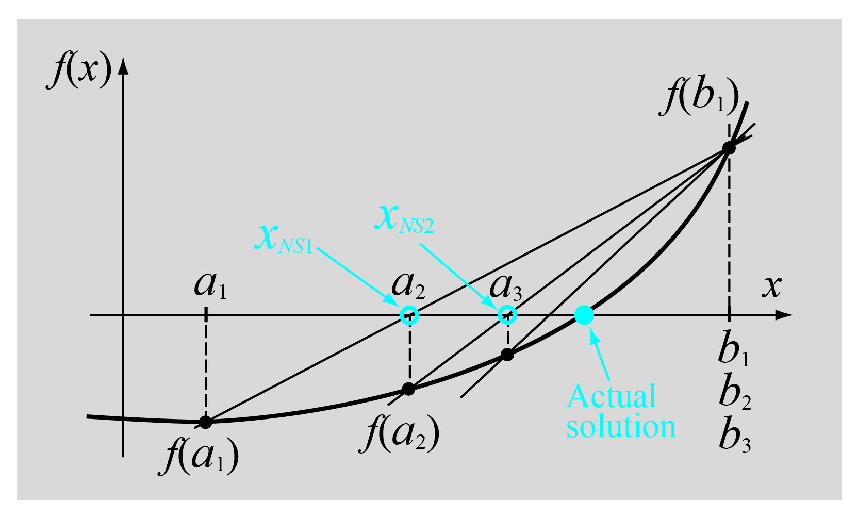
\includegraphics{Chapter3_Fig3_9.eps}
\caption{The first two iterations of the regula falsi method.}
\label{fig:lec3n-regula-falsi}
\end{marginfigure}
The straight line connecting $f(a)$ to $f(b)$ is given by Equation \ref{eq:lec3n-regula-falsi}:
\begin{equation}
y = \frac{f(b) - f(a)}{b-a}(x-b)+f(b)
\label{eq:lec3n-regula-falsi}
\end{equation}
The point where the line intersects the $x$-axis is found by setting $y=0$ and solving for $x$, giving us:
\begin{equation}
x_{\text{NS}} = \frac{a f(b) - b f(a)}{f(b) - f(a)}
\label{eq:lec3n-regula-falsi-xns}
\end{equation}
The algorithm for the regula falsi method is as follows:
\begin{enumerate}
\item Find an interval $[a,b]$ in which a root exists.  One way to find such an interval is to identify an $a$ and $b$ for which $f(a)f(b)<0$.
\item Use Equation \ref{eq:lec3n-regula-falsi-xns} to find the new estimate of the numerical solution.
\item Determine whether the root is in $[a,x_{\text{NS}}]$ or in $[x_{\text{NS}},b]$ using the following method:
\begin{itemize}
\item If $f(a)f(x_{\text{NS}}) < 0$, the root is in $[a,x_{\text{NS}}]$.
\item If $f(x_{\text{NS}})f(b) < 0$, the root is in $[x_{\text{NS}},b]$.
\end{itemize}
\item Select the subinterval that contains the solution---either $[a,x_{\text{NS}},b]$ or $[x_{\text{NS}},b]$ as determined in step 3---as the new $a$ and $b$ and return to step 2.
\end{enumerate}
The iteration should be stopped when the estimated error is smaller than the pre-determined tolerance.  Some notes on this method:
\begin{itemize}
\item Like the bisection method, the regula falsi method \emph{will} converge.  One can hope that, given the small added complexity, the rate of convergence would be somewhat faster using the regula falsi method.
\item For a given function, it is typically the case that only one endpoint will ``move towards'' the solution.  Modifications to the algorithm can be made to address this issue and will be considered in the assignments.
\end{itemize}
